\subsection{Organización del Proyecto y Comunicación}

La estructura de participantes del Kit Pagos Colombia es más acotada que la de proyectos con clientes externos o múltiples grupos de interés. El equipo de desarrollo no negocia entregas con un stakeholder ni valida funcionalidades con usuarios en campo.

El proyecto tiene adicionalmente dependencias técnicas con las cuatro pasarelas de pago analizadas en la fase de identificación. Estas entidades no intervienen activamente en el proceso; la relación con ellas es unidireccional: el equipo consume sus portales de documentación y entornos sandbox, sin coordinación humana directa bajo condiciones normales.

\subsubsection{Interfaces Externas}

\begin{center}
\renewcommand{\arraystretch}{1.2}
\begin{longtable}{|P{0.243}|P{0.241}|P{0.241}|P{0.241}|}
  \hline
  Nombre de la entidad & Descripción & Responsabilidades en el proyecto & Datos de contacto / medio de comunicación. \\
  \hline
  \endfirsthead
  \hline
  Nombre de la entidad & Descripción & Responsabilidades en el proyecto & Datos de contacto / medio de comunicación. \\
  \hline
  \endhead
  \caption{Interfaces Externas}
  \label{tab:interfaces-externas}\\
  \endlastfoot
  Ph.D. Jaime Andrés Pavlich Mariscal & Director del trabajo de grado. Profesor titular del Departamento de Ingeniería de Sistemas de la Pontificia Universidad Javeriana & Supervisión de la ejecución teniendo en cuenta lo establecido en la metodología. Aprobación de entregables clave; retroalimentación sobre decisiones arquitectónicas y criterios de evaluación; lineamientos académicos generales. & jpavlich@\allowbreak javeriana.edu.co / Ext. 4731 / Reuniones presenciales o virtuales acordadas durante el semestre. \\
  \hline
  Pontificia Universidad Javeriana & Institución académica en la que se desarrolla el proyecto & Marco institucional del trabajo de grado; derechos de uso académico sobre el documento final; acceso a recursos y plataformas institucionales & Canales institucionales de la universidad \\
  \hline
  Wompi (Bancolombia) & Pasarela de pago colombiana operada por Bancolombia, uno de los cuatro proveedores integrados en el framework & Provee documentación técnica de su API REST, entorno sandbox y datos de prueba utilizados en la fase de análisis, desarrollo y evaluación & \href{http://docs.wompi.co}{docs.wompi.co} \\
  \hline
  Rapyd (que adquirió PayU GPO) & Plataforma de pagos global con operación en Colombia, uno de los cuatro proveedores integrados en el framework. En marzo de 2025 compró la operación de PayU GPO en América Latina, y el proyecto la integra en lugar de PayU (punto 15 del registro de arquitectura) & Provee documentación técnica de su API, entorno sandbox y datos de prueba & \href{https://docs.rapyd.net}{docs.rapyd.net} \\
  \hline
  Mercado Pago & Pasarela de origen argentino con operación en Colombia y varios países de latinoamérica, uno de los cuatro proveedores integrados en el framework & Provee documentación técnica de su API, entorno sandbox y datos de prueba & \href{http://developers.mercadopago.com}{developers.\allowbreak mercadopago.com} \\
  \hline
  Kushki & Plataforma latinoamericana con operación activa en Colombia, uno de los cuatro proveedores integrados en el framework & Provee documentación técnica de su API, entorno sandbox y datos de prueba & \href{https://docs.kushki.com}{docs.kushki.com} \\
  \hline
\end{longtable}
\end{center}

Toda interacción relevante con estas entidades quedará registrada en actas o bitácoras. La comunicación con las pasarelas de pago ocurre exclusivamente a través de sus portales públicos; el contacto directo con equipos de soporte se reserva para situaciones que lo justifiquen y que no puedan resolverse por documentación.

\subsubsection{Organigrama y Descripción de Roles}

A diferencia de esquemas con rotación de roles por sprint, se adoptaron asignaciones estables que reflejan las especializaciones técnicas del framework: un componente de arquitectura y núcleo, cuatro adaptadores de pasarela con una API de simulación, y un proceso de evaluación con métricas de código.

Cada integrante lidera uno de esos frentes sin dejar de contribuir a los demás, especialmente durante la fase de desarrollo iterativo, es decir que todos deben aportar a cada entregable de manera equitativa, independientemente su responsabilidad principal dentro de lo establecido a continuación.

La jerarquía en el nivel operativo es plana. El coordinador del equipo no tiene autoridad técnica sobre los demás sino responsabilidad sobre la gestión del backlog, el calendario y la comunicación con el director. Las decisiones técnicas se toman por consenso entre los integrantes involucrados en el frente correspondiente.

\begin{figure}[H]
  \centering
  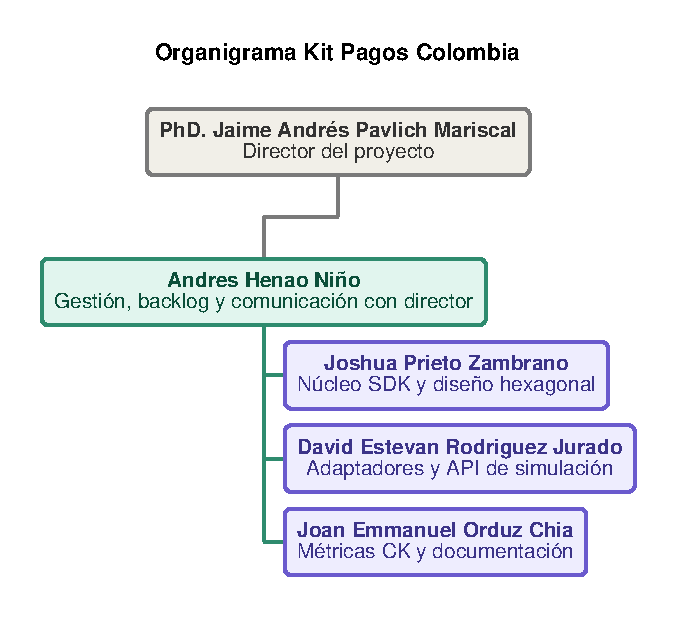
\includegraphics[width=\textwidth]{figuras/02-organigrama}
  \caption{Organigrama del equipo de trabajo.}
  \label{fig:organigrama}
\end{figure}

\begin{center}
\renewcommand{\arraystretch}{1.2}
\begin{longtable}{|P{0.25}|P{0.25}|P{0.25}|P{0.25}|}
  \hline
  \textbf{Integrante} & \textbf{Rol} & \textbf{Descripción} & \textbf{Responsabilidades} \\
  \hline
  \endfirsthead
  \hline
  \textbf{Integrante} & \textbf{Rol} & \textbf{Descripción} & \textbf{Responsabilidades} \\
  \hline
  \endhead
  \caption{Descripción de los roles.}
  \label{tab:roles}\\
  \endlastfoot
  Ph.D. Jaime Andrés Pavlich Mariscal & Director del Proyecto & Supervisor académico externo al equipo. No participa en la implementación técnica & Aprobación de entregables clave, retroalimentación sobre arquitectura, métricas de evaluación y alcance del framework \\
  \hline
  Andres Henao Niño & Coordinador del equipo & Integrante responsable de la gestión operativa del proyecto. Participa activamente en el desarrollo & Mantenimiento del backlog y seguimiento del calendario; coordinación de reuniones internas; comunicación con el director; registro de actas y decisiones clave \\
  \hline
  Joshua Prieto Zambrano & Líder de arquitectura y núcleo SDK & Responsable del diseño estructural del framework y la implementación del núcleo & Diseño del modelo de dominio unificado; especificación de los puertos de la arquitectura hexagonal; implementación del núcleo del SDK; revisión de que los adaptadores cumplan los contratos de puerto \\
  \hline
  David Estevan Rodriguez Jurado & Líder de integración & Responsable de los cuatro adaptadores por pasarela y de la API de simulación & Implementación de los adaptadores de Wompi, Rapyd, Mercado Pago y Kushki; desarrollo y despliegue de la API de simulación; consolidación de la documentación de datos de prueba \\
  \hline
  Joan Emmanuel Orduz Chia & Líder de evaluación y documentación & Integrante responsable del proceso de medición con métricas CK, los proyectos prototípicos y el documento final & Diseño y ejecución de la evaluación comparativa con métricas WMC, CBO y RFC; desarrollo de los prototipos de medición; redacción del documento de grado y publicación del repositorio público \\
  \hline
\end{longtable}
\end{center}

Los canales de comunicación del equipo son cuatro. La coordinación diaria entre los integrantes va por un grupo de WhatsApp, y las reuniones con el director, los lunes de 2 a 3 p.~m., por videoconferencia en Microsoft Teams. El backlog y el seguimiento de tareas se llevan en los hitos y los issues de GitHub. El control de versiones y la revisión de código también se hacen en GitHub, con pull requests para todo cambio sobre \texttt{devops} y \texttt{main}.
